%modification history
% 9 jul 2011
% 29 nov 2011

\documentclass[11pt, letterpaper]{article}
\usepackage[margin=1in]{geometry}

% \documentclass[11pt, letterpaper]{article}
%
% % ----- margins -----
%
% \topmargin -1.5cm         % read Lamport p.163
% \oddsidemargin -0.04cm    % read Lamport p.163
% \evensidemargin -0.04cm   % same as oddsidemargin but for left-hand pages
%
% % ----- texts -----
%
% \textwidth 16.59cm
% \textheight 21.94cm
%
% % ----- indendts and spacing -----
%
% \parskip 0pt            	% spacing between paragraphs
% %\renewcommand{\baselinestretch}{1.5}	% uncomment for 1.5 spacing
%
% \parindent 7mm		      % leading space for paragraphs between lines
%
% % ----- page # -----
%
% %\pagestyle{empty}         % uncomment if don't want page numbers





\usepackage{amsfonts, amsmath, amssymb, amsthm}
\usepackage{graphicx}

%modification history
% 2012
% May 3

%=== use the these packages if they are not already in use ===
%\usepackage{amsfonts, amsmath, amssymb, amsthm}
%=============================================================

%===== fonts =====
\def\ttt{\texttt}
%===== spacing =====

\def\extraspacing{\vspace{2mm} \noindent}
\def\figcapup{\vspace{-1mm}}
\def\figcapdown{\vspace{-0mm}}
\def\hgap{\textrm{\hspace{1mm}}}
\def\thmvgap{\vspace{0mm}}
\def\vgap{\vspace{2mm}}


%===== tabbing =====

\def\tab{\hspace{3mm}}
\def\tabpos{\hspace{4mm} \= \hspace{4mm} \= \hspace{4mm} \= \hspace{4mm} \=
\hspace{4mm} \= \hspace{4mm} \= \hspace{4mm} \= \hspace{4mm} \= \hspace{4mm}
\kill}

%===== blocks =====

\newtheorem{theorem}{Theorem}
\newtheorem{lemma}{Lemma}
\newtheorem{corollary}{Corollary}
\newtheorem{proposition}{Proposition}
\newtheorem{definition}{Definition}
\newtheorem{problem}{Problem}

%===== math macros =====

\def\bm{\boldmath}
\def\defeq{\stackrel{\textrm{\tiny{def}}}{=}}
\def\eps{\epsilon}
\def\fr{\frac}
\def\-{\mbox{-}}
\def\inte{\mathbb{N}}
\def\ovline{\overline}
\def\real{\mathbb{R}}

\def\lc{\lceil}
\def\lf{\lfloor}
\def\rc{\rceil}
\def\rf{\rfloor}

\def\nn{\nonumber}

\def\Pr{\mathbf{Pr}}
\def\expt{\mathbf{E}}
\def\var{\mathbf{var}}

\def\*{\star}

\DeclareMathOperator*{\argmin}{arg\,min}
\DeclareMathOperator*{\polylg}{polylg}
\DeclareMathOperator*{\polylog}{polylog}
\DeclareMathOperator*{\intr}{\cap}

%===== misc =====

\def\done{\hspace*{\fill} $\framebox[2mm]{}$}	% end of proof
%\def\done{\hspace*{\fill} $\Box$}	% end of proof

%===== coloring =====

\newcommand{\red}[1]{\textcolor{red}{#1}}

\begin{document}

\noindent These are the questions from Yufei's lecture.

\extraspacing {\bf Question 1 (5\%).} Given two points $o, o'$, let us define that $o$ {\em dominates} $o'$ if the coordinate of $o$ is smaller than that of $o'$ on each dimension. By this definition, what is the skyline of the dataset shown in the figure below?

\begin{center}
    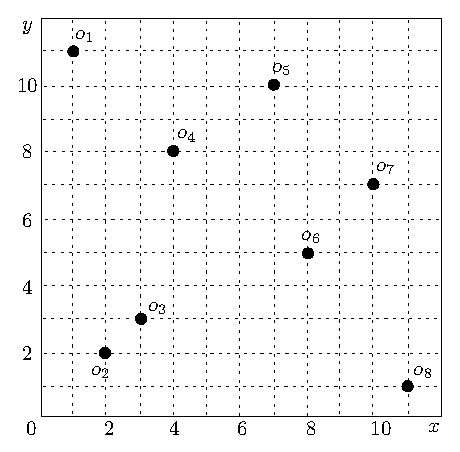
\includegraphics[height=60mm]{./artwork/ds.eps}
\end{center}

\noindent {\bf Answer:} $\{o_1, o_2, o_8\}$.

\extraspacing {\bf Question 2 (5\%).} Recall that the {\em SFS} algorithm works by first sorting all the data points according to a scoring function $f(x, y)$. Let the function be $f(x, y) = x$. For example, a point $(5, 4)$ has score 5. In other words, {\em SFS} processes the data points in ascending order of their scores. For each point $o$, its processing requires comparing $o$ to some other points. In the dataset shown in the above figure, when point $o_3$ is being processed, which point or points is $o_3$ compared to?

\extraspacing {\bf Answer:} $\{o_1, o_2\}$.

\end{document}
